% ENGLISH TEMPLATE: FIGURE AND CITATION EXAMPLES
% !TeX program = xelatex
% GENERIC RESEARCH PROJECT TEMPLATE
% Overleaf: main.tex + XeLaTeX.
% Keep all four .tex files in the same folder.
% Add a logos/ subfolder for partner images.
% Each cover has editable logo blocks A, B and C.
% INSPIRE is active; BI0S alternatives are commented.
% Settings: see preamble.tex.
% After migrating from biblatex, use
% Recompile from scratch.
\documentclass[a4paper,12pt]{article}
% ENGLISH TEMPLATE: BIBLIOGRAPHY FIX
% PREAMBLE
% Compile main.tex with XeLaTeX.
% Keep one option active in each settings group.

% LANGUAGE
% English (default):
\usepackage[brazilian,english]{babel}
% Brazilian Portuguese (replace the line above):
% \usepackage[english,brazilian]{babel}
%
% The last language is the main language.
% Babel sets hyphenation and automatic labels.
% Translate your own headings and text manually.
% For a short passage in another language:
% \foreignlanguage{brazilian}{Portuguese text}
% For a longer passage:
% \begin{otherlanguage}{brazilian}
% [Your Portuguese text here.]
% \end{otherlanguage}

% FONT
\usepackage{fontspec}
\setmainfont{Linux Libertine O}
% Use XeLaTeX, not pdfLaTeX.
% Do not load inputenc or fontenc here.

% MARGINS
% These are template design choices.
\usepackage[
  a4paper,
  margin=2.5cm,
  headheight=15pt,
  footskip=1.2cm
]{geometry}

% LINE SPACING
\usepackage{setspace}
% FAPESP scholarship projects: double spacing.
\doublespacing
% General use: replace the line above with:
% \onehalfspacing
% Or, for single spacing:
% \singlespacing
%
% Check the rules for your specific funding call.
% This setting is not universal FAPESP compliance.
% General scholarship guidance:
% https://fapesp.br/253/projeto-de-pesquisa
% Body size: 12 pt, set in main.tex.
% Cover pages use local single spacing.

% PARAGRAPHS
% Indented, with no extra space between paragraphs:
\usepackage{indentfirst}
\setlength{\parindent}{1.25cm}
\setlength{\parskip}{0pt}
% Alternative: replace the two settings above.
% \setlength{\parindent}{0pt}
% \setlength{\parskip}{0.6em}

% GRAPHICS AND COVER COLORS
\usepackage{graphicx}
\graphicspath{{logos/}{fig/}}
\usepackage[table,svgnames]{xcolor}
\usepackage{tikz}
\usetikzlibrary{
  calc,intersections,decorations.text
}
\definecolor{feecDarkBlue}{HTML}{00427A}
\definecolor{feecNavy}{HTML}{102B4E}
\definecolor{feecPurple}{HTML}{562877}
\definecolor{feecGreen}{HTML}{B0D361}
\definecolor{feecLavender}{HTML}{EACCFF}
% Color names are inherited from the original cover.

% COVER B COLORS
% Original attachment omitted these definitions.
% These editable defaults match the shared palette.
\definecolor{aimsBlue}{HTML}{00427A}
\definecolor{aimsYellow}{HTML}{F2C94C}
\definecolor{aimsTeal}{HTML}{238A8D}

% FUTURE COVERS
% Add new named colors and TikZ libraries here.
% Put each design in its own titlepage_*.tex file.
% Do not change global fonts/spacing for one cover.

% TABLES, FIGURES AND MATHEMATICS
\usepackage{array}
\usepackage{tabularx}
\usepackage{booktabs}
\usepackage{longtable}
\usepackage{float}
\usepackage{caption}
\usepackage{subcaption}
\usepackage{amsmath,amssymb}
\usepackage{enumitem}
\captionsetup{font=small,labelfont=bf}
\renewcommand{\arraystretch}{1.2}
\setcounter{secnumdepth}{3}
\setcounter{tocdepth}{2}

% LINKS
% Load BEFORE abntex2cite.
% abntex2cite detects hyperref when it loads.
\usepackage{hyperref}
\hypersetup{
  colorlinks=true,
  linkcolor=feecDarkBlue,
  citecolor=feecDarkBlue,
  urlcolor=feecDarkBlue
}

% ABNT AUTHOR-DATE CITATIONS
% Keep this package for either document language.
% It provides native \citeonline support.
\usepackage[alf]{abntex2cite}
% Do not also load cite, natbib or biblatex.
% The package selects abntex2-alf automatically.
% Do not add another \bibliographystyle command.
%
% Replace 'key' with a real entry from your .bib:
% According to \citeonline{key}, ...
% ... \cite{key}.
% \citeonline[p.~25]{key}
% \cite[p.~25]{key}
% \cite{key1,key2}
%
% Enable the bibliography at the end of main.tex.
% Use BibTeX, not Biber.
% Local compilation sequence:
% 1. xelatex main
% 2. bibtex main
% 3. xelatex main
% 4. xelatex main
% Overleaf runs these steps automatically.
%
% After switching from biblatex/Biber, use:
% Recompile from scratch.
% This clears incompatible .aux and .bbl files.
% The package uses the traditional abnTeX2 style.
% Later ABNT revisions are not applied automatically.

% FOOTER
% Language-neutral page numbering.
\usepackage{fancyhdr}
\usepackage{lastpage}
\pagestyle{fancy}
\fancyhf{}
\renewcommand{\headrulewidth}{0pt}
\renewcommand{\footrulewidth}{0.4pt}
\fancyfoot[R]{%
  \small\color{black!70}%
  \thepage\ / \pageref{LastPage}}
\fancypagestyle{plain}{%
  \fancyhf{}
  \renewcommand{\headrulewidth}{0pt}
  \renewcommand{\footrulewidth}{0.4pt}
  \fancyfoot[R]{%
    \small\color{black!70}%
    \thepage\ / \pageref{LastPage}}}


% PROJECT DETAILS
% Replace these values for each new project.
% Edit the fields below for each new project.

\newcommand{\projectTitle}{Research Project Title}
\newcommand{\subprojectTitle}{%
  Project subtitle or brief description}
\newcommand{\docsubtitle}{Research Project}
\newcommand{\applicantName}{Applicant name}
\newcommand{\leadResearcher}{%
  Lead researcher name}
\newcommand{\hostInstitution}{Host institution name}
\newcommand{\hostDepartment}{School or department name}
\newcommand{\fundingAgency}{%
  Funding agency or program name}
\newcommand{\grantNumber}{%
  To be completed, if applicable}
\newcommand{\projectPeriod}{Month/year to month/year}
\newcommand{\docdate}{Month year}
\newcommand{\projectCity}{City}
% For Portuguese, change babel in preamble.tex.
% Translate these values and your headings manually.
\hypersetup{
  pdftitle={\projectTitle},
  pdfauthor={\applicantName}
}

\begin{document}

% COVER GALLERY
% Both covers are active for comparison.
% Keep ONE input line for the final document.
% Delete or comment out the unwanted input line.
% COVER A: FLOWING CURVES -- PUBLIC DEFAULT
% Lower logos always use the bottom-left corner.
% All logo widths enlarged by 25 percent.
% Include from main.tex; do not compile alone.
% Uses shared project fields from main.tex.
% Keep all cover formatting inside titlepage.

\begin{titlepage}
  \thispagestyle{empty}
  \singlespacing
  \begin{tikzpicture}[remember picture,overlay]
    \draw[feecPurple,line width=12pt,opacity=0.30]
      ([xshift=-5cm]current page.north)
      to[out=-70,in=140] ([yshift=6cm]current page.east);
    \draw[feecLavender,line width=7pt,opacity=0.50]
      ([xshift=-4cm]current page.north)
      to[out=-70,in=140] ([yshift=5cm]current page.east);
    \draw[feecNavy,line width=10pt,opacity=0.25]
      ([xshift=5cm]current page.south)
      to[out=100,in=-30] ([yshift=-5cm]current page.west);
    \draw[feecGreen,line width=6pt,opacity=0.40]
      ([xshift=4cm]current page.south)
      to[out=100,in=-30] ([yshift=-4cm]current page.west);

    \node at (current page.center)
      [text width=0.76\paperwidth,
       align=center,inner sep=0pt] {%
      \begin{minipage}{0.76\paperwidth}
        \centering
        \setlength{\parskip}{0pt}
        \setlength{\parindent}{0pt}
        {\color{feecNavy}\fontsize{25}{31}%
          \selectfont\bfseries
          \projectTitle\par}
        \vspace{0.7cm}
        {\color{feecDarkBlue}\fontsize{16}{21}%
          \selectfont
          \subprojectTitle\par}
        \vspace{1cm}
        {\color{feecDarkBlue}\fontsize{14}{19}%
          \selectfont
          \docsubtitle\par}
        \vspace{2cm}
        {\fontsize{13}{18}\selectfont
          \applicantName\par}
        \vspace{0.5cm}
        {\fontsize{12}{16}\selectfont
          Lead researcher: \leadResearcher\par}
        \vspace{1cm}
        {\color{black!70}\fontsize{12}{16}%
          \selectfont
          \hostInstitution\par
          \hostDepartment\par}
        \vspace{0.7cm}
        {\color{black!70}\fontsize{12}{16}%
          \selectfont
          \projectCity, \docdate\par}
      \end{minipage}};
    % LOGO ARRANGEMENTS
    % Keep ONE complete block active.
    % Comment its nodes before enabling another.
    % Widths preserve each image aspect ratio.
    % Keep files in the shared logos/ folder.
    % Always include UNICAMP, FEEC and AIMS files.
    % Partner options need extra logo files.

    % DEFAULT: INSTITUTIONS + PARTNER PLACEHOLDER
    % UNICAMP, FEEC and AIMS remain visible.
    % Only the partner/project logo changes.
    % Replace logo-placeholder.png with your logo,
    % or activate one of the partner blocks below.
    % Keep ONE complete configuration active.
    \node[anchor=north east,inner sep=0pt]
      at ([xshift=-1.5cm,yshift=-1.5cm]
        current page.north east) {%
      \raisebox{-0.5\height}{%
        
\includegraphics[width=2.375cm]
          {logos/logo-unicamp.png}}%
      \hspace{0.65cm}%
      \raisebox{-0.5\height}{%
        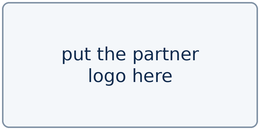
\includegraphics[width=3.75cm]
          {logos/logo-placeholder.png}}%
    };
    \node[anchor=south west,inner sep=0pt]
      at ([xshift=1.5cm,yshift=1.3cm]
        current page.south west) {%
      \raisebox{-0.5\height}{%
        
\includegraphics[width=4.125cm]
          {logos/logo-feec.png}}%
      \hspace{0.65cm}%
      \raisebox{-0.5\height}{%
        
\includegraphics[width=3.125cm]
          {logos/logo-aims-branco-texto.png}}%
    };

    % A: INSPIRE / CPQD
    % Add the named images to logos/ first.
    % Uncomment both nodes to use this option.
    % \node[anchor=north east,inner sep=0pt]
    %   at ([xshift=-1.5cm,yshift=-1.5cm]
    %     current page.north east) {%
    %   \raisebox{-0.5\height}{%
    %     \includegraphics[width=2.375cm]
    %       {logos/logo-unicamp.png}}%
    %   \hspace{0.65cm}%
    %   \raisebox{-0.5\height}{%
    %     \includegraphics[width=3.75cm]
    %       {logos/logo-cpqd.png}}%
    % };
    % \node[anchor=south west,inner sep=0pt]
    %   at ([xshift=1.5cm,yshift=1.3cm]
    %     current page.south west) {%
    %   \raisebox{-0.5\height}{%
    %     \includegraphics[width=4.125cm]
    %       {logos/logo-feec.png}}%
    %   \hspace{0.65cm}%
    %   \raisebox{-0.5\height}{%
    %     \includegraphics[width=3.125cm]
    %       {logos/logo-aims-branco-texto.png}}%
    % };

    % B: BI0S
    % Uncomment all nodes in this block.
    % \node[anchor=north east,inner sep=0pt]
    %   at ([xshift=-1.5cm,yshift=-1.5cm]
    %     current page.north east) {%
    %   \raisebox{-0.5\height}{%
    %     \includegraphics[width=2.375cm]
    %       {logos/logo-unicamp.png}}%
    %   \hspace{0.65cm}%
    %   \raisebox{-0.5\height}{%
    %     \includegraphics[width=3.75cm]
    %       {logos/logo-bi0s.png}}%
    % };
    % \node[anchor=south west,inner sep=0pt]
    %   at ([xshift=1.5cm,yshift=1.3cm]
    %     current page.south west) {%
    %   \raisebox{-0.5\height}{%
    %     \includegraphics[width=4.125cm]
    %       {logos/logo-feec.png}}%
    %   \hspace{0.65cm}%
    %   \raisebox{-0.5\height}{%
    %     \includegraphics[width=3.125cm]
    %       {logos/logo-aims-branco-texto.png}}%
    % };

    % C: BI0S + CEB
    % Uncomment all nodes in this block.
    % Three unit/group logos share the lower row.
    % \node[anchor=north east,inner sep=0pt]
    %   at ([xshift=-1.5cm,yshift=-1.5cm]
    %     current page.north east) {%
    %   \raisebox{-0.5\height}{%
    %     \includegraphics[width=2.375cm]
    %       {logos/logo-unicamp.png}}%
    %   \hspace{0.65cm}%
    %   \raisebox{-0.5\height}{%
    %     \includegraphics[width=3.75cm]
    %       {logos/logo-bi0s.png}}%
    % };
    % \node[anchor=south west,inner sep=0pt]
    %   at ([xshift=1.5cm,yshift=1.3cm]
    %     current page.south west) {%
    %   \raisebox{-0.5\height}{%
    %     \includegraphics[width=4.125cm]
    %       {logos/logo-feec.png}}%
    %   \hspace{0.65cm}%
    %   \raisebox{-0.5\height}{%
    %     \includegraphics[width=3.125cm]
    %       {logos/logo-aims-branco-texto.png}}%
    %   \hspace{0.65cm}%
    %   \raisebox{-0.5\height}{%
    %     \includegraphics[width=2.75cm]
    %       {logos/logo-ceb.png}}%
    % };

    % FUTURE PARTNERS
    % Copy a block and update names/positions.
    % Use one width per logo; do not force height.

  \end{tikzpicture}
\end{titlepage}


% COVER B: GEOMETRIC ARCS -- PUBLIC DEFAULT
% BI0S width: 3.6 cm (20 percent larger).
% The three-logo lower row starts 0.8 cm from left.
% Include from main.tex; do not compile alone.
% Uses shared project fields from main.tex.
% Colors and TikZ libraries live in preamble.tex.

\begin{titlepage}
  \thispagestyle{empty}
  \singlespacing
  \begin{tikzpicture}[overlay,remember picture]
    % Main arc and its reference point.
    \draw[ultra thick,aimsBlue,name path=big arc]
      ([xshift=-2mm]current page.north)
      arc(150:285:11)
      coordinate[pos=0.225] (x0);

    \begin{scope}
      % Clip the pattern to the upper-right corner.
      \clip ([xshift=-2mm]current page.north)
        arc(150:285:11) -- (current page.north east);

      % Background circles.
      \fill[feecPurple!10]
        ([xshift=4.55cm]x0) circle (4.55);
      \fill[feecGreen!25]
        ([xshift=3.40cm]x0) circle (3.40);
      \fill[aimsYellow!40]
        ([xshift=2.25cm]x0) circle (2.25);

      % Secondary arcs.
      \draw[ultra thick,aimsBlue]
        (x0) arc(-90:30:6.5);
      \draw[ultra thick,aimsBlue]
        (x0) arc(90:-30:8.75);
      \draw[very thick,aimsTeal!70,name path=arc1]
        (x0) arc(90:-90:4.675);
      \draw[very thick,aimsTeal!60]
        (x0) arc(90:-90:2.875);

      % Geometric intersections.
      \path[name intersections={
        of=big arc and arc1,by=x1}];
      \draw[ultra thick,aimsBlue,name path=arc2]
        (x1) arc(135:-20:4.75);
      \draw[very thick,aimsTeal!70]
        (x1) arc(135:-20:8.75);
      \path[name intersections={
        of=big arc and arc2,by={aux,x2}}];
      \draw[very thick,aimsTeal!65]
        (x2) arc(180:50:2.25);
    \end{scope}

    % Curved institution label.
    % Use plain text in the hostInstitution field.
    \path[decorate,decoration={
      text along path,
      text color=aimsBlue,
      raise=-2.8ex,
      text/.expanded={|\noexpand\bfseries|%
        \hostInstitution},
      text align=center
    }] ([xshift=-2mm]current page.north)
      arc(150:245:11);

    % Lower decorative curves.
    \draw[feecPurple,line width=10pt,opacity=0.25]
      ([xshift=3cm]current page.south)
      to[out=100,in=-30]
      ([yshift=-9.5cm]current page.west);
    \draw[feecGreen,line width=6pt,opacity=0.40]
      ([xshift=2.5cm]current page.south)
      to[out=100,in=-30]
      ([yshift=-9cm]current page.west);

    % Upper-left identification block.
    \node[anchor=west,align=left,text width=7cm]
      at ([xshift=2.5cm,yshift=3cm]
        current page.west) {%
      {\color{feecNavy}\LARGE\bfseries
        \docsubtitle\par}
      \vspace{0.5cm}
      {\color{feecNavy}\large
        \fundingAgency\par}
      \vspace{0.4cm}
      {\color{feecNavy}\large
        \projectPeriod\par}
    };

    % Title and subtitle.
    \node[align=center,text width=0.76\paperwidth]
      at ([yshift=-3.5cm]current page.center) {%
      {\color{feecDarkBlue}\LARGE\bfseries
        \projectTitle\par}
      \vspace{0.3cm}
      {\color{feecDarkBlue}\large
        \subprojectTitle\par}
    };

    % Applicant and department.
    \node[align=center,text width=0.76\paperwidth]
      at ([yshift=-6.5cm]current page.center) {%
      {\large\applicantName\par}
      {\large\hostDepartment\par}
      \vspace{0.3cm}
      {Lead researcher: \leadResearcher\par}
    };

    % Date and location.
    \node[anchor=south east,align=right]
      at ([xshift=-2cm,yshift=1.5cm]
        current page.south east) {%
      \color{black!70}\large
      \projectCity\\
      \docdate
    };

    % LOGO ARRANGEMENTS
    % Keep ONE complete block active.
    % Comment its nodes before enabling another.
    % Widths preserve each image aspect ratio.
    % Keep files in the shared logos/ folder.
    % Always include UNICAMP, FEEC and AIMS files.
    % Partner options need extra logo files.

    % DEFAULT: INSTITUTIONS + PARTNER PLACEHOLDER
    % UNICAMP, FEEC and AIMS remain visible.
    % Only the partner/project logo changes.
    % Replace logo-placeholder.png with your logo,
    % or activate one of the partner blocks below.
    % Keep ONE complete configuration active.
    \node[anchor=north west,inner sep=0pt]
      at ([xshift=1.5cm,yshift=-1.5cm]
        current page.north west) {%
      \raisebox{-0.5\height}{%
        
\includegraphics[width=1.9cm]
          {logos/logo-unicamp.png}}%
      \hspace{0.65cm}%
      \raisebox{-0.5\height}{%
        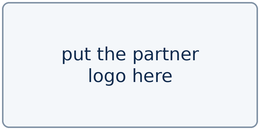
\includegraphics[width=3.0cm]
          {logos/logo-placeholder.png}}%
    };
    \node[anchor=south west,inner sep=0pt]
      at ([xshift=1.5cm,yshift=1.3cm]
        current page.south west) {%
      \raisebox{-0.5\height}{%
        
\includegraphics[width=3.3cm]
          {logos/logo-feec.png}}%
      \hspace{0.65cm}%
      \raisebox{-0.5\height}{%
        
\includegraphics[width=2.5cm]
          {logos/logo-aims-branco-texto.png}}%
    };

    % A: INSPIRE / CPQD
    % Add the named images to logos/ first.
    % Uncomment both nodes to use this option.
    % \node[anchor=north west,inner sep=0pt]
    %   at ([xshift=1.5cm,yshift=-1.5cm]
    %     current page.north west) {%
    %   \raisebox{-0.5\height}{%
    %     \includegraphics[width=1.9cm]
    %       {logos/logo-unicamp.png}}%
    %   \hspace{0.65cm}%
    %   \raisebox{-0.5\height}{%
    %     \includegraphics[width=3.0cm]
    %       {logos/logo-cpqd.png}}%
    % };
    % \node[anchor=south west,inner sep=0pt]
    %   at ([xshift=1.5cm,yshift=1.3cm]
    %     current page.south west) {%
    %   \raisebox{-0.5\height}{%
    %     \includegraphics[width=3.3cm]
    %       {logos/logo-feec.png}}%
    %   \hspace{0.65cm}%
    %   \raisebox{-0.5\height}{%
    %     \includegraphics[width=2.5cm]
    %       {logos/logo-aims-branco-texto.png}}%
    % };

    % B: BI0S
    % Uncomment all nodes in this block.
    % \node[anchor=north west,inner sep=0pt]
    %   at ([xshift=1.5cm,yshift=-1.5cm]
    %     current page.north west) {%
    %   \raisebox{-0.5\height}{%
    %     \includegraphics[width=1.9cm]
    %       {logos/logo-unicamp.png}}%
    %   \hspace{0.65cm}%
    %   \raisebox{-0.5\height}{%
    %     \includegraphics[width=3.6cm]
    %       {logos/logo-bi0s.png}}%
    % };
    % \node[anchor=south west,inner sep=0pt]
    %   at ([xshift=1.5cm,yshift=1.3cm]
    %     current page.south west) {%
    %   \raisebox{-0.5\height}{%
    %     \includegraphics[width=3.3cm]
    %       {logos/logo-feec.png}}%
    %   \hspace{0.65cm}%
    %   \raisebox{-0.5\height}{%
    %     \includegraphics[width=2.5cm]
    %       {logos/logo-aims-branco-texto.png}}%
    % };

    % C: BI0S + CEB
    % Uncomment all nodes in this block.
    % Three unit/group logos share the lower row.
    % \node[anchor=north west,inner sep=0pt]
    %   at ([xshift=1.5cm,yshift=-1.5cm]
    %     current page.north west) {%
    %   \raisebox{-0.5\height}{%
    %     \includegraphics[width=1.9cm]
    %       {logos/logo-unicamp.png}}%
    %   \hspace{0.65cm}%
    %   \raisebox{-0.5\height}{%
    %     \includegraphics[width=3.6cm]
    %       {logos/logo-bi0s.png}}%
    % };
    % \node[anchor=south west,inner sep=0pt]
    %   at ([xshift=0.8cm,yshift=1.3cm]
    %     current page.south west) {%
    %   \raisebox{-0.5\height}{%
    %     \includegraphics[width=3.3cm]
    %       {logos/logo-feec.png}}%
    %   \hspace{0.65cm}%
    %   \raisebox{-0.5\height}{%
    %     \includegraphics[width=2.5cm]
    %       {logos/logo-aims-branco-texto.png}}%
    %   \hspace{0.65cm}%
    %   \raisebox{-0.5\height}{%
    %     \includegraphics[width=2.2cm]
    %       {logos/logo-ceb.png}}%
    % };

    % FUTURE PARTNERS
    % Copy a block and update names/positions.
    % Use one width per logo; do not force height.

  \end{tikzpicture}
\end{titlepage}


% ADD MORE COVER DESIGNS HERE
% 1. Copy a cover into titlepage_new.tex.
% 2. Keep one titlepage environment in that file.
% 3. Reuse the project fields defined above.
% 4. Keep font and spacing changes local.
% 5. Add any packages/colors to preamble.tex.
% 6. Uncomment its input below to preview it.
% \input{titlepage_new.tex}

% The information sheet below is independent.
% Keep or remove it according to your needs.

% PROJECT INFORMATION
% Remove rows that do not apply.
\begin{titlepage}
  \thispagestyle{empty}
  \singlespacing
  \vspace*{1.5cm}
  \begin{center}
    {\color{feecNavy}\Large\bfseries
      Project Information\par}
    \vspace{1.4cm}
    \renewcommand{\arraystretch}{1.5}
    \begin{tabularx}{0.95\linewidth}{@{}
      >{\raggedright\arraybackslash\bfseries}
      p{0.30\linewidth}X@{}}
      Title: & \projectTitle \\
      Document: & \docsubtitle \\
      Applicant: & \applicantName \\
      Lead researcher: & \leadResearcher \\
      Host institution: & \hostInstitution \\
      Unit: & \hostDepartment \\
      Funding: & \fundingAgency \\
      Process: & \grantNumber \\
      Period: & \projectPeriod \\
      Date: & \docdate \\
    \end{tabularx}
  \end{center}
  \vfill
  \begin{center}
    \projectCity\par
    \docdate
  \end{center}
\end{titlepage}

% MAIN TEXT
% Numbering restarts here. This does not exempt
% the cover pages from a funding body's page limit.
\pagenumbering{arabic}
\pagestyle{fancy}

% ABSTRACT: centered on its own page.
% General FAPESP scholarship limit: 20 lines.
\clearpage
\thispagestyle{empty}
\null
\vfill
\begin{abstract}
[Summarize the problem, objectives, methods, and
expected results.]
\end{abstract}
\vfill
\null
\clearpage

% OPTIONAL CONTENTS PAGE
% \tableofcontents
% \clearpage

\section{Introduction and Motivation}
[Present the research problem, its relevance, and the
key literature.]

\subsection{Background}
[Introduce the concepts and context needed to
understand the problem.]

\subsection{Research Gap}
[Identify the limitations of existing work and the
intended contribution.]

% OPTIONAL RESEARCH CENTER AFFILIATION
% \subsection{Research Center Affiliation}
% [Explain the alignment and contributions.]

\section{Objectives}
[State the main objective and the specific objectives.]

\section{Materials and Methods}
[Describe the research design, materials, data, and
procedures.]

\subsection{Resources and Infrastructure}
[Describe the available resources and additional
requirements.]

\subsection{Research Procedures}
[Describe the research steps and methods, including
ethical considerations.]

\subsection{Analysis of Results}
[Define metrics, evaluation criteria, and analysis
procedures.]

\section{Work Plan and Schedule}
[List the activities, milestones, deliverables, and
deadlines.]

\section{Expected Results}
[Describe the expected scientific contributions and
outputs.]

% TEACHING EXAMPLES
% Remove this section before submitting a project.
% Keep your own images in fig/ and logos in logos/.
\section{Template Examples: Figures and Citations}

\subsection{An intentionally fictional reference}
% First citation and first entry in references.bib.
% The author name also places it first alphabetically.
The first example is deliberately fictional:
\citeonline{aardvark2026fictional} wrote
\emph{This Reference Does Not Exist: Cite It and Your
Career May Become Fiction Too}. Neither the author
nor the book is real. This template Easter egg is a
reminder to verify every reference, especially those
suggested by an AI tool. Remove this paragraph and
the fictional entry before submitting your work.

\subsection{Academic writing and research habits}
% Narrative citation: author is part of the sentence.
\citeonline{booth2024craft} discuss research questions,
evidence, and the construction of arguments.
\citeonline{belcher2019writing} provides a structured
workbook for developing a journal article.
% Parenthetical citation: author/year in parentheses.
A regular writing schedule is also a useful topic
for graduate researchers to explore
\cite{silvia2018write}.

\subsection{Organizing graduate research}
\citeonline{allen2015getting} presents an approach to
organizing commitments and next actions, while
\citeonline{newport2016deep} discusses protecting time
for demanding, focused work. These general-purpose
books can inform a graduate student's work habits;
they are not substitutes for a research methodology
or a guarantee of productivity.

\subsection{Including and referencing a figure}
Figure~\ref{fig:ml-research-lifecycle} presents the
\emph{Machine Learning Research Lifecycle}, a teaching
framework for academic research. It connects research
questions, study design, model development, evaluation,
publication, and follow-up research. Inspired by the
iterative approach of CRISP-ML(Q)
\cite{studer2021crisp}, it emphasizes scientific
contributions rather than business deployment.
This is a new educational adaptation, not an
established standard or a figure from the cited paper.

% Store research images in fig/.
% Set width only to preserve the aspect ratio.
% Keep the label after the caption.
\begin{figure}[htbp]
  \centering
  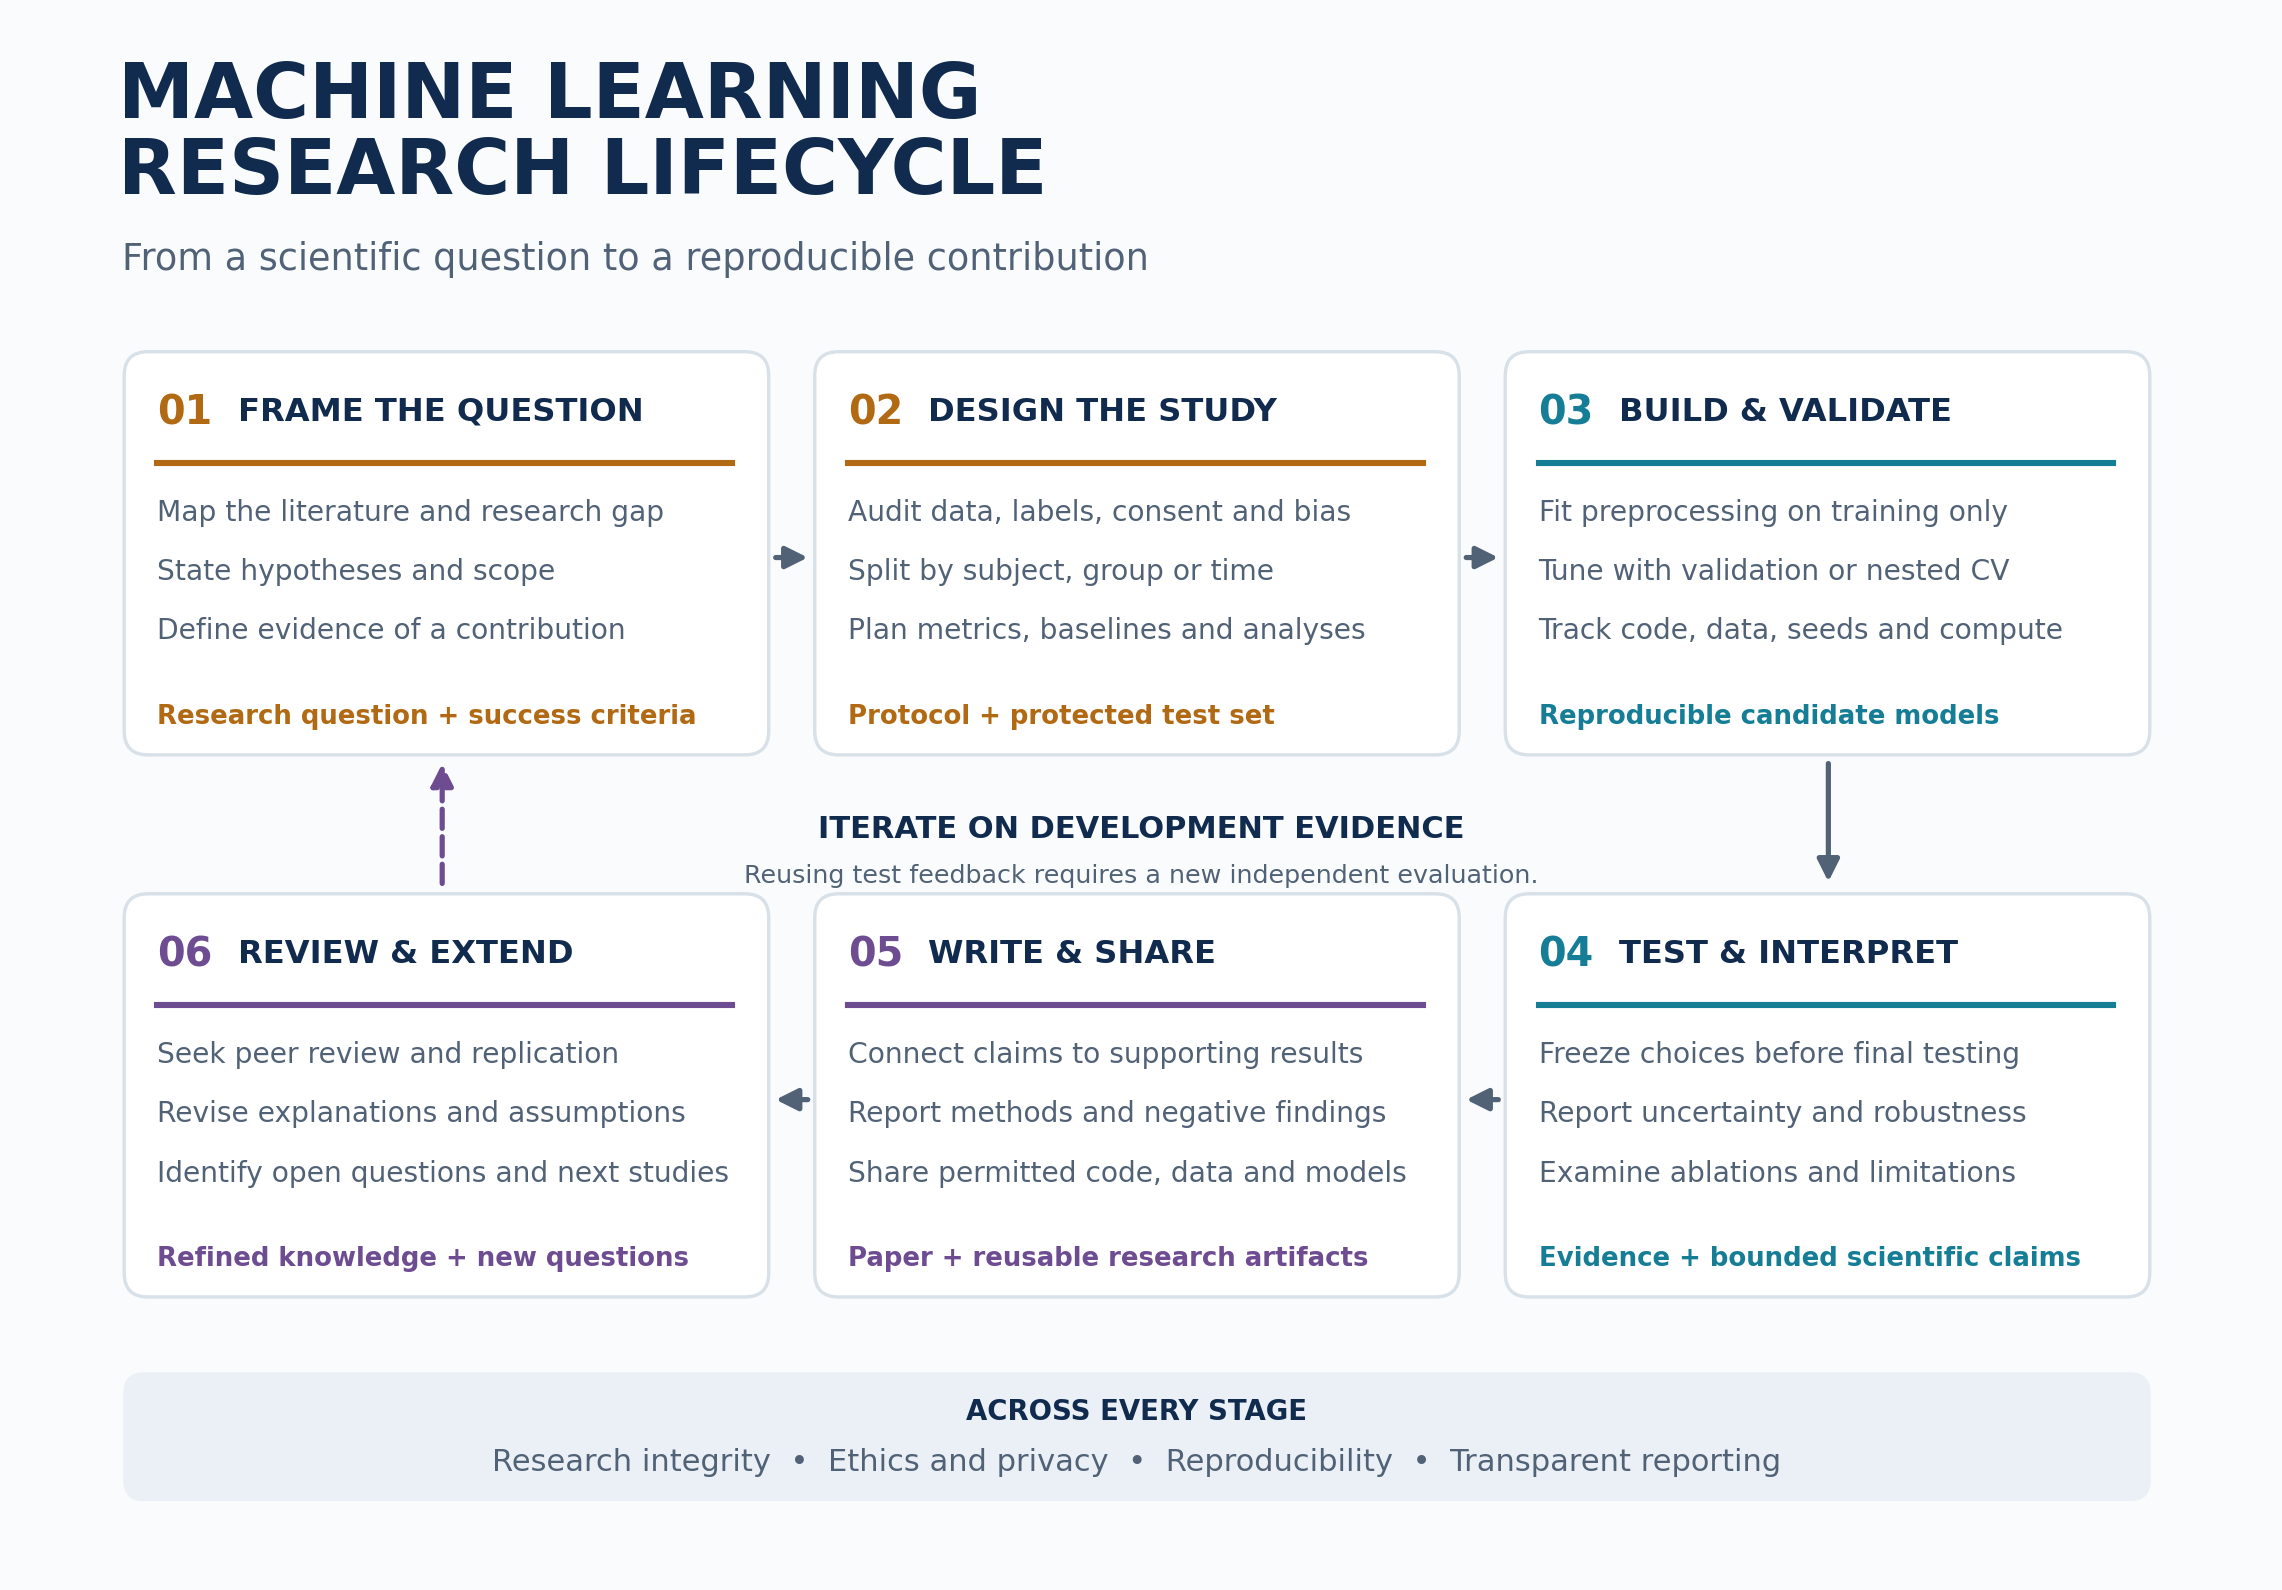
\includegraphics[width=\linewidth]
    {fig/ml_research_lifecycle.png}
  \caption{Machine Learning Research Lifecycle.
    Original educational diagram created for this
    template, inspired by CRISP-ML(Q)
    \cite{studer2021crisp} and adapted to academic
    research. The stages are iterative; test data
    must remain independent of model selection.}
  \label{fig:ml-research-lifecycle}
\end{figure}

% BIBLIOGRAPHY
% Uses abntex2cite from the existing preamble.
% BibTeX reads references.bib (no extension here).
% Only cited entries are printed.
% If switching from biblatex, recompile from scratch.
\clearpage
\bibliography{references}

\end{document}
